
\thispagestyle{empty}

\newpage
{\Large \bf

  \noindent Supplementary Material\\

  \noindent 
 Effects of Tunable Hydrophobicity on the Collective Hydrodynamics of Janus Particles under Flows}\\

\noindent 
Szu-Pei Fu$^{1,*},$ 
Rolf Ryham$^{2},$ 
Bryan Quaife$^{3}$ and Y.-N. Young$^{4},$
\\

\noindent
$^{1}$Department of Mathematics, Trinity College, Hartford, Connecticut 06106, USA

\noindent
$^{2}$Department of Mathematics, Fordham University, Bronx, NY, USA

\noindent
$^{3}$Department of Scientific Computing, Florida State University, Tallahassee, Florida 32306, USA

\noindent
$^{4}$Department of Mathematical Sciences, New Jersey Institute of Technology, Newark, NJ 07102 USA
\\

\noindent $^*$Corresponding author. Address: Department of Mathematics, Trinity College, 
300 Summit Street, Hartford, CT 06106. email: \text{peter.fu@trincoll.edu}



\setcounter{page}{1}

\setcounter{figure}{0}
\renewcommand{\thefigure}{S\arabic{figure}}

\setcounter{equation}{0}
\renewcommand{\theequation}{S\arabic{equation}}

\setcounter{section}{0}
\renewcommand{\thesection}{S\arabic{section}} 


%-----ellipse repulsion--------------------

%\Phi_{\mathrm{rep}}

\section{Movie Descriptions}
We consider suspensions of JPs of radius 1.25~nm. The time step size for
all simulations is $\Delta t = 0.2$~ns. The colors of the JPs are as
follows: for Type I and Vesicles, red is hydrophobic ($\max g > 0$) and
blue is hydrophilic ($\min g = 0$); for Type II, red is more hydrophobic
($\max g >0$) than blue ($\min g > 0$); for Type III, red is positively
charged ($\max g > 0$) and blue is negatively charged ($\min g < 0$).
%\mbox{} \\

\noindent
{\bf Relaxation}: The relaxation of 60 circular JPs that are initialized
with random locations and orientations. The JPs self-assemble into
unilamellar (Type I), multilamellar (Type II), and striated (Type III)
configurations. The final configurations are used as initial conditions
for the simulations that include a background flow. 

%There are 60 circular particles with radius 1.25~nm that are initially
%confined in a square box. The simulation results show the relaxation
%with each of the three boundary conditions. The time step of all
%simulations is $\Delta t=0.2$. The color on the boundary from blue to
%red is for $\min g(\xx)$ to $\max g(\xx)$. All final configurations are
%adopted in simulations with hydrodynamic flows. \\


\noindent
{\bf Structures in a Weak Shear Flow}:
The relaxed configurations of the 60 JPs are subjected to a weak shear
flow. The shear rate is $\dot{\gamma} = 0.05$~ns$^{-1}$ for the Vesicle,
Type I, and Type II configurations, and $\dot{\gamma} = 0.1$~ns$^{-1}$
for the Type III configuration. The vesicle undergoes tank-treading and
the bilayer increases its orientational order. The multilamellar
configuration resembles a rigid body motion, and the striated
configuration has an even stronger resemblance to a rigid body motion.
No ruptures occur in these examples. 

%We adopt the relaxed configurations and place the JP structures in the
%shear flow. For the choices of the shear rate, we pick: $\dot\gamma =
%0.05$ ns$^{-1}$ for the vesicle, $\dot\gamma = 0.05$ ns$^{-1}$ for the
%bilayer, $\dot\gamma = 0.05$ ns$^{-1}$ for the multi-lamellar, and
%$\dot\gamma = 0.1$ ns$^{-1}$ for the striated configurations. The
%vesicle case undergoes tank-treading whereas the initially disordered
%BC (i) case increases orientational order. The multilamellar assemply
%behaves as a rigid body, and the striated configuration moreso. No
%ruptures occur. \\

\noindent
{\bf Structures in a Weak Taylor-Green Flow}:
The relaxed configurations of the 60 JPs are subjected to a weak
Taylor-Green flow. The flow rate is $\dot{\gamma} = 0.05$~ns$^{-1}$ for
the Vesicle, Type I, and Type II configurations, and $\dot{\gamma} =
0.1$~ns$^{-1}$ for the Type III configuration. The vesicle stays intact,
whereas the bilayer is pulled apart into different TG cells. Like in the
weak shear flow example, the multilamellar and striated configurations
behave as rigid bodies.

%For the choices of the flow strength, we pick: $\dot\gamma = 0.05$
%ns$^{-1}$ for the vesicle, $\dot\gamma = 0.05$ ns$^{-1}$ for the
%disordered bilayer, $\dot\gamma = 0.05$ ns$^{-1}$ for the
%multi-lamellar, and $\dot\gamma = 0.1$ ns$^{-1}$ for the striated
%configurations. The vesicle stays inact, whereas the dissordered
%bilayer is pulled apart. Like in Supplementary Movie S2, the striated
%assembly is basically rigid. \\

%We adopt the relaxed configurations and place the JP structures in the
%Taylor-Green flow at low flow rates. For the choices of the flow
%strength, we pick: $\dot\gamma = 0.05$ ns$^{-1}$ for the vesicle,
%$\dot\gamma = 0.05$ ns$^{-1}$ for the disordered bilayer, $\dot\gamma =
%0.05$ ns$^{-1}$ for the multi-lamellar, and $\dot\gamma = 0.1$
%ns$^{-1}$ for the striated configurations. The vesicle stays inact,
%whereas the dissordered bilayer is pulled apart. Like in Supplementary
%Movie S2, the striated assembly is basically rigid. \\


\noindent
{\bf Structures in a Strong Shear Flow}:
The relaxed configurations of the 60 JPs are subjected to a strong shear
flow. The shear rate is $\dot{\gamma} = 0.075$~ns$^{-1}$ for the Vesicle
configuration, $\dot{\gamma} = 0.1$~ns$^{-1}$ for the Type I
configuration, and $\dot{\gamma} = 0.15$~ns$^{-1}$ for the Type II and
Type III configurations. In all cases, the structure is ruptured by the
flow. The frames are stabilized by moving with the center of mass of all
the JPs.

%We adopt the relaxed configurations and place the JP structures in the
%shear flow at a higher shear rate. For the choices of the shear rate, we
%pick: $\dot\gamma = 0.075$ for the vesicle, $\dot\gamma = 0.1$ ns$^{-1}$
%for the bilayer, $\dot\gamma = 0.15$ ns$^{-1}$ for the multi-lamellar,
%and $\dot\gamma = 0.15$ ns$^{-1}$ for the striated configurations. The
%time step of all simulations is $\Delta t=0.2$ ns$^{-1}$. In this movie,
%some clear structural ruptures occur in each case. In order to observe
%the structure behaviors at later time, we stabilize the frame by
%tracking the center of mass position of all JP. \\

\noindent
{\bf Structures in a Strong Taylor-Green Flow}:
The relaxed configurations of the 60 JPs are subjected to a strong
Taylor-Green flow. The flow rate is $\dot{\gamma} = 0.1$~ns$^{-1}$ for
the Vesicle, Type I, and Type II configurations, and $\dot{\gamma} =
0.15$~ns$^{-1}$ for the Type III configuration. In all cases, the
structure is ruptured by the flow and there is a significant reduction
in the orientation order. While the Vesicle Type I configurations are
broken into several pieces, the main body of the Type II and Type III
configurations are not pulled apart by the background flow.

%We adopt the relaxed configurations and place the JP structures in the
%Taylor-Green flow at higher flow rates. For the choices of the flow
%strength, we pick: $\dot\gamma = 0.1$ ns$^{-1}$ for the vesicle, $\dot\gamma = 0.1$ ns$^{-1}$ for the
%bilayer, $\dot\gamma = 0.1$ ns$^{-1}$ for the multi-lamellar, and $\dot\gamma = 0.15$ ns$^{-1}$ for the
%striated configurations. Clear structural ruptures occur in each case.
%In all cases, there is significant reduction in the orientational order
%of the assemblies. While the BC (i) cases are broken into several
%pieces, the main body of the BC (ii) and BC (iii) assemblies are not
%pulled apart by the background flow.\\

\noindent
%{\label{MovieS6}\bf JP Vesicle in a Taylor-Green Flow with Various
%$\lambda$ Values}: 
{\label{MovieS6}\bf JP Vesicle in Various Taylor-Green Flows}: A
circular vesicle bilayer is placed in a Taylor-Green flow. The parameter
$\lambda$ controls the TG cell size and the values are varied from 1~nm
to 4~nm while the flow rate is chosen so that
$\lambda\dot\gamma=0.1$~nm/ns. The parameter $\lambda$ determines the
steady-state polygonal tank-treading shape. The rotation direction is
clockwise for $\lambda=1$~nm and $\lambda=2$~nm, and counterclockwise
for $\lambda=3$~nm and $\lambda=4$~nm. Streamlines of the flow are
included.

%A circular vesicle bilayer is placed in the Taylor-Green flow.  The
%parameter $\lambda$ controls the cell size and the values are varied
%from 1.0 nm to 4.0 nm while the flow rate $\lambda\dot\gamma=0.1$ is
%fixed. There is a rotation transition from clockwise ($\lambda=1$ nm and
%2 nm) to counterclockwise ($\lambda=3$ nm and 4 nm). Moreover, the
%resulting steady shapes of all cases are different polygons. We plot the
%streamlines in the background.\\


\section{Raw Data}
The following figures plot the fully resolved simulation time-courses
organized in terms of the bilayer, vesicle BL, multilamellar, and striated JP phases
under shear flow (Supplementary Figures~\ref{fig:ulshraw}--\ref{fig:stshraw})
and under TG flow (Supplementary Figures~\ref{fig:ultgraw}--\ref{fig:sttgraw}).
Throughout, panels (a) are for relative free energy $F - F_0$,
panels (b) for alignment $S_2$, and panels (c) for strain $E$ (as a percentage). 
A common ordinate is used for each of the respective panels to facilitate
comparison between data sets. 
%\newpage

\begin{figure}[h!]
\begin{center}
\textbf{\textsc{Shear Flow cases}}\par\medskip
\textbf{Type I, bilayer phase under shear flow}\par\medskip
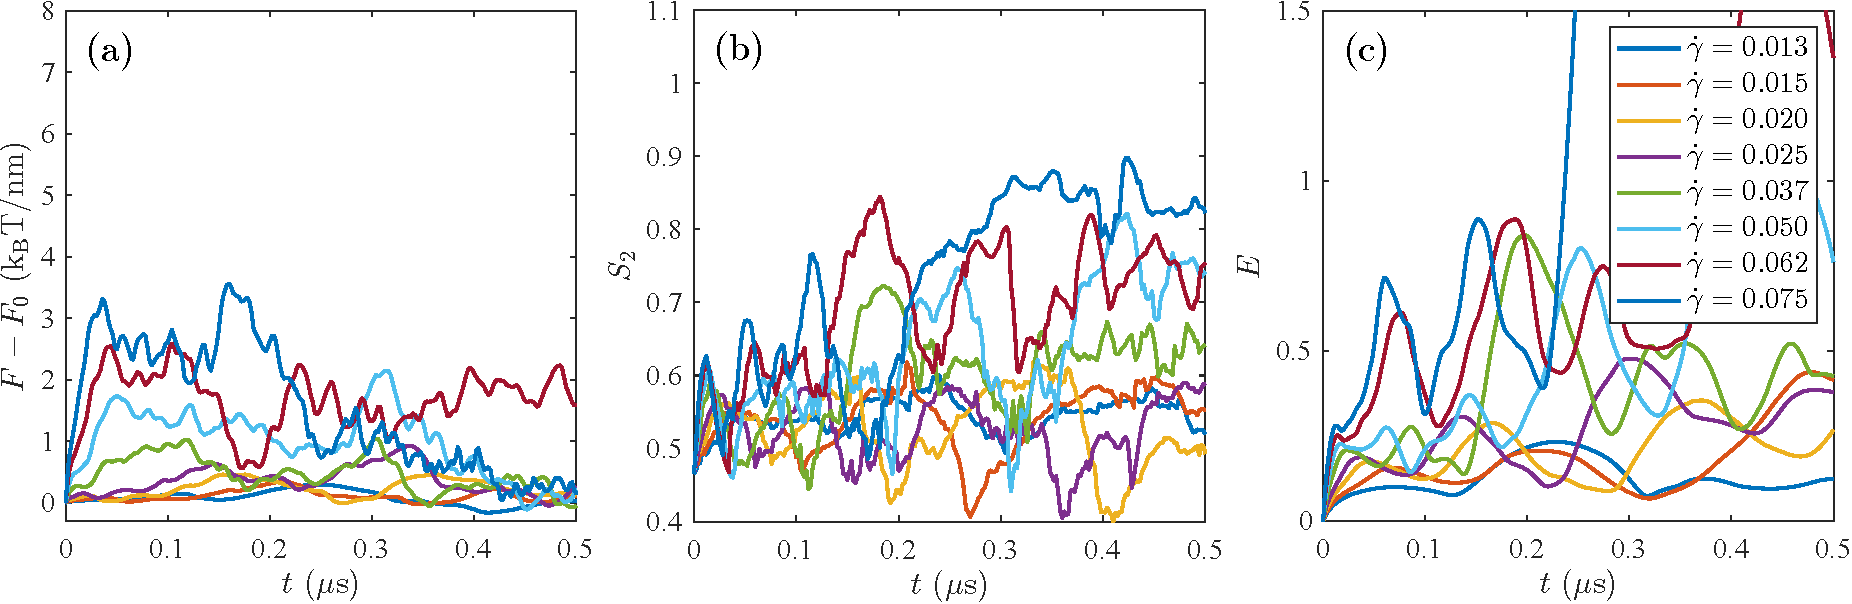
\includegraphics[width=\textwidth]{SMFigures/ULShRaw.pdf}
\end{center}
\caption{
Relative free energy $F - F_0$,
alignment $S_2$, and strain $E$ for
Type I, bilayer phase under shear flow with choices of shear rates $\dot\gamma=0.013$ -- $0.075$ ns$^{-1}$.
%The change in free energy $F$ is plotted in panel (a). Panel (b) shows the scalar order parameter $S_2$ over time $t$. Panel (c) plots the change of strain parameter $E$ in percentage over time $t$.
}
\label{fig:ulshraw}
\end{figure}


\begin{figure}[h!]
\begin{center}
\textbf{Type I, vesicle BL phase under shear flow}\par\medskip
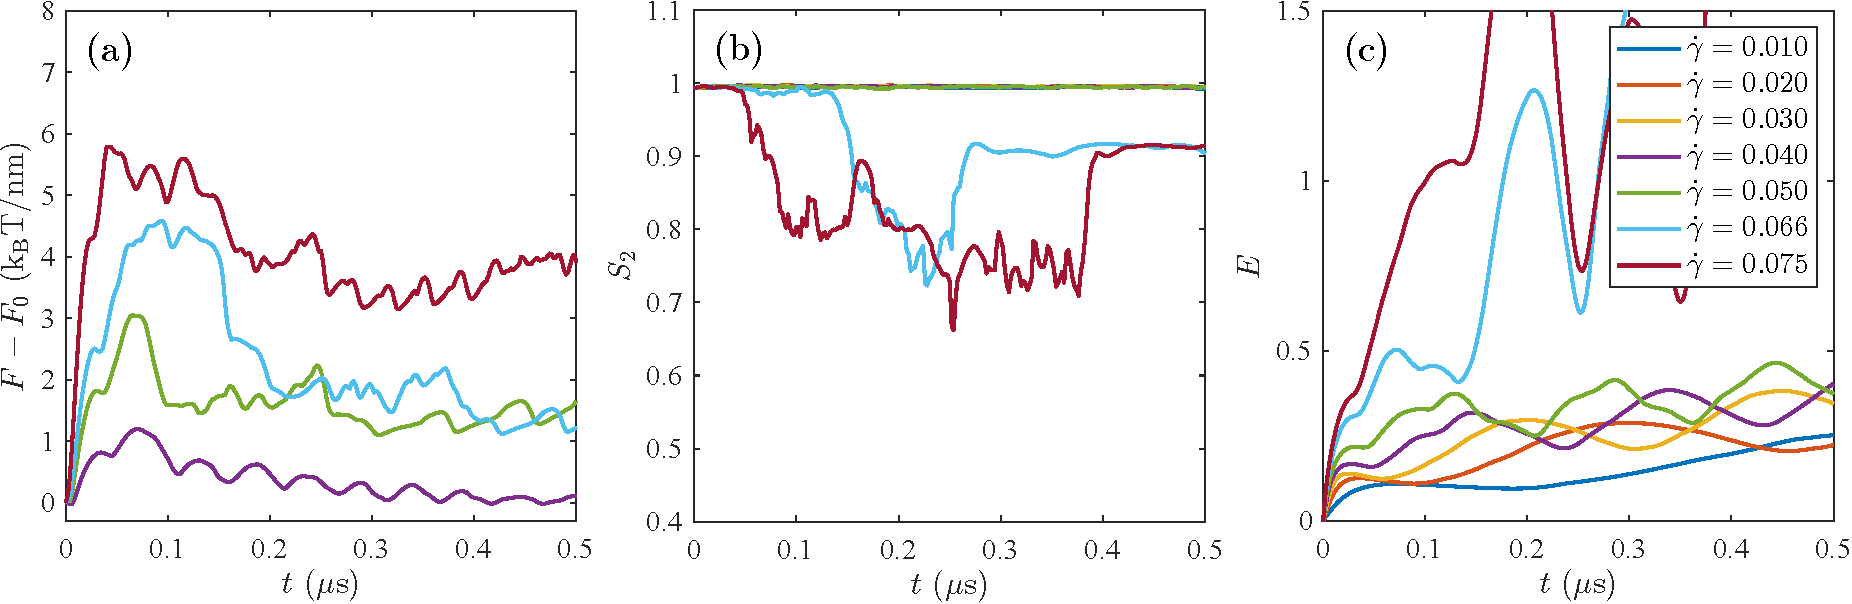
\includegraphics[width=\textwidth]{SMFigures/VeShRaw.pdf}
\end{center}
\caption{
Relative free energy $F - F_0$,
alignment $S_2$, and strain $E$ for
Type I, bilayer phase under shear flow with choices of shear rates $\dot\gamma=0.01$ -- $0.075$ ns$^{-1}$.
The JP type is the same as for Supplementary Figure \ref{fig:ulshraw} but with a
ring-shaped, rather than disordered, bilayer for initial configuration.  
%A Vesicle under a shear flow with choices of shear rates $\dot\gamma=0.01\sim0.075$. The change in free energy $F$ is plotted in panel (a). Panel (b) shows the scalar order parameter $S_2$ over time $t$. Panel (c) plots the change of strain parameter $E$ in percentage over time $t$.
}
\label{fig:veshraw}
\end{figure}


\begin{figure}[h!]
\textbf{Type II, multilamellar phase under shear flow}\par\medskip
\begin{center}
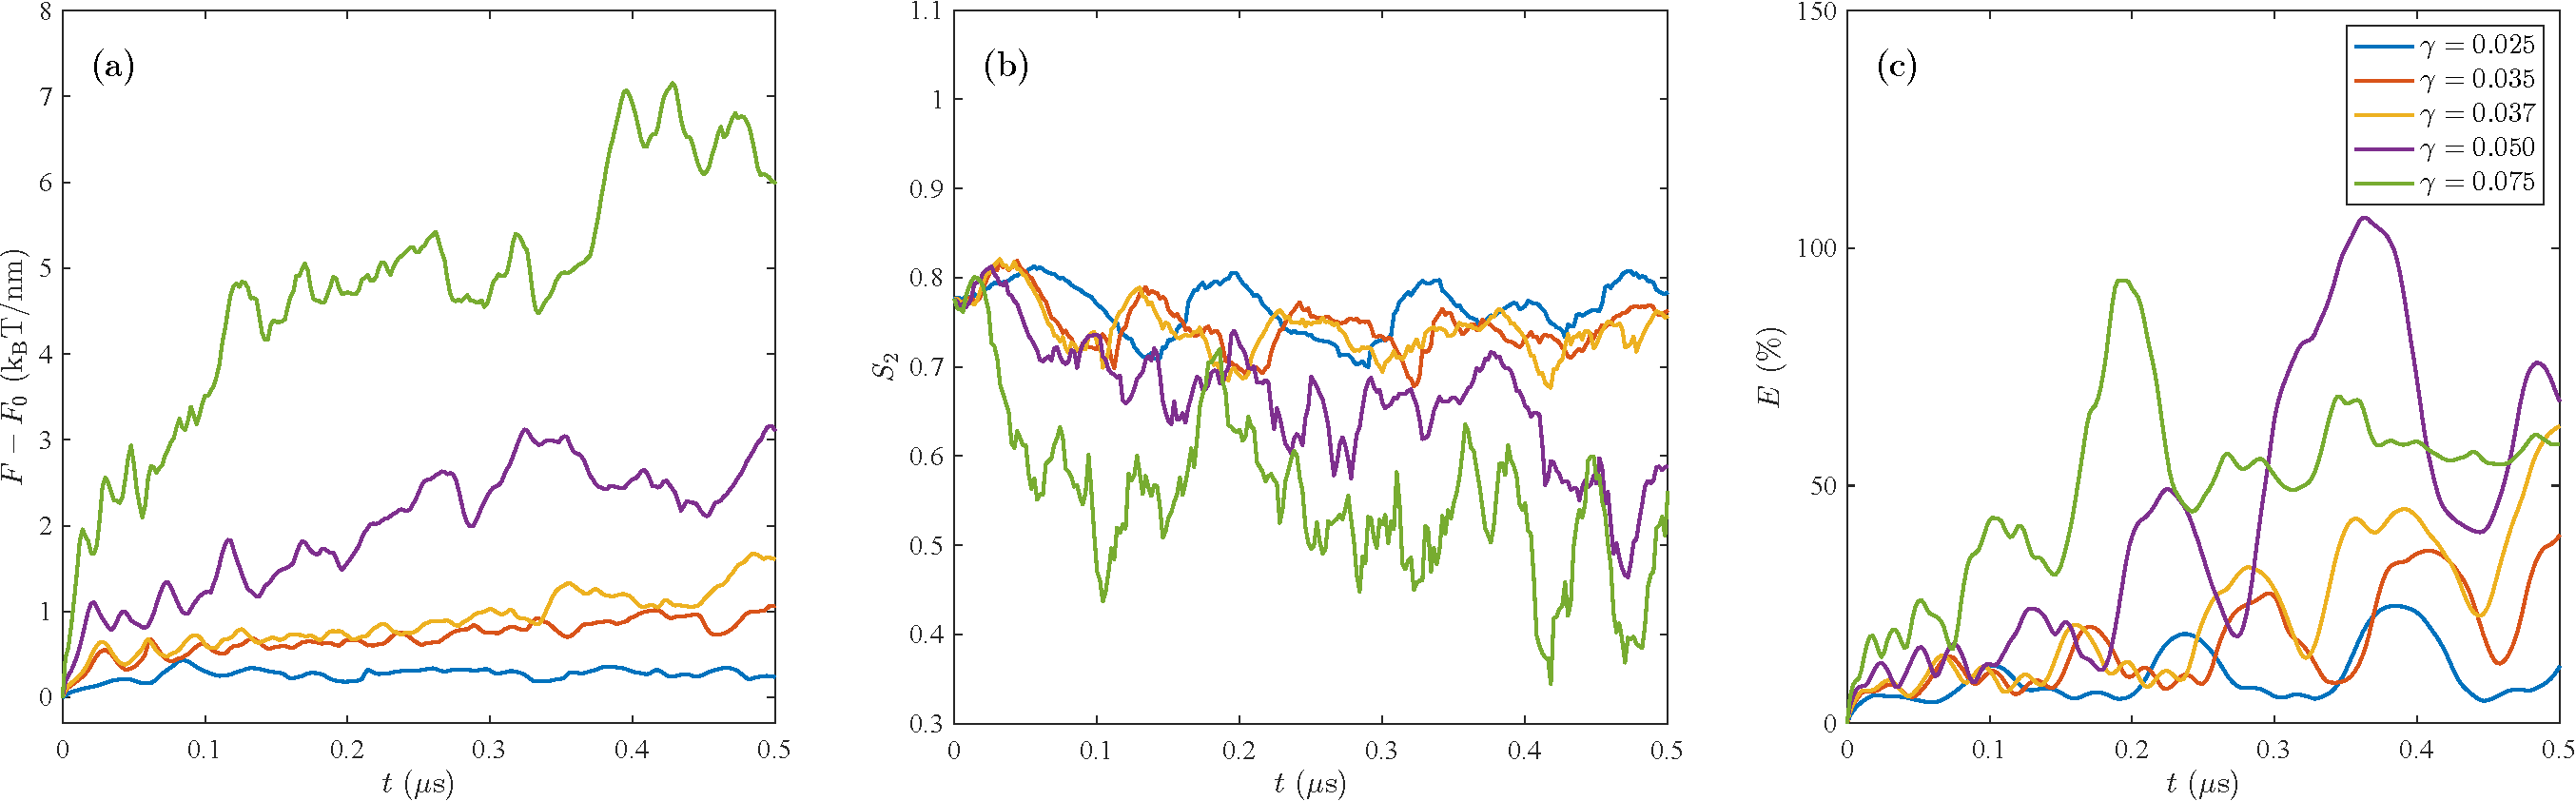
\includegraphics[width=\textwidth]{SMFigures/MLShRaw.pdf}
\end{center}
\caption{
Relative free energy $F - F_0$,
alignment $S_2$, and strain $E$ for
Type II, multilamellar phase under shear flow with choices of shear rates $\dot\gamma=0.025$ -- $0.075$ ns$^{-1}$.
%A multilamellar JP structure under a shear flow with choices of shear rates $\dot\gamma=0.025\sim0.075$. The change in free energy $F$ is plotted in panel (a). Panel (b) shows the scalar order parameter $S_2$ over time $t$. Panel (c) plots the change of strain parameter $E$ in percentage over time $t$.
}
\label{fig:mlshraw}
\end{figure}


\begin{figure}[h!]
\textbf{Type III, striated phase under shear flow}\par\medskip
\begin{center}
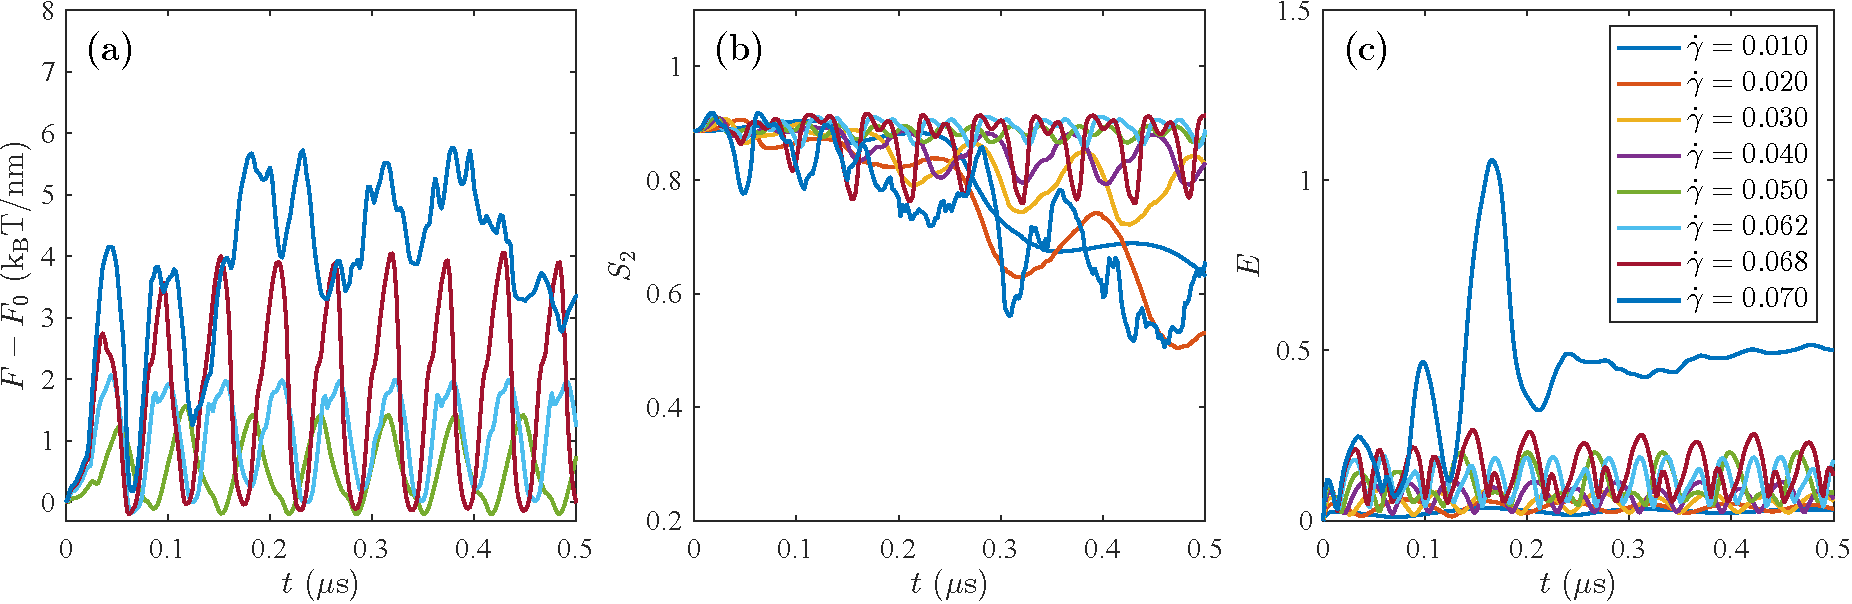
\includegraphics[width=\textwidth]{SMFigures/StShRaw.pdf}
\end{center}
\caption{
Relative free energy $F - F_0$,
alignment $S_2$, and strain $E$ for
Type III, striated phase under shear flow with choices of shear rates $\dot\gamma=0.01$ -- $0.07$ ns$^{-1}$.
%A striated JP structure under a shear flow with choices of shear rates $\dot\gamma=0.01\sim0.07$. The change in free energy $F$ is plotted in panel (a). Panel (b) shows the scalar order parameter $S_2$ over time $t$. Panel (c) plots the change of strain parameter $E$ in percentage over time $t$.
}
\label{fig:stshraw}
\end{figure}

\begin{figure}[h!]
\begin{center}
\textbf{\textsc{TG Flow Cases}}\par\medskip
\textbf{Type I, bilayer  phase under TG flow}\par\medskip
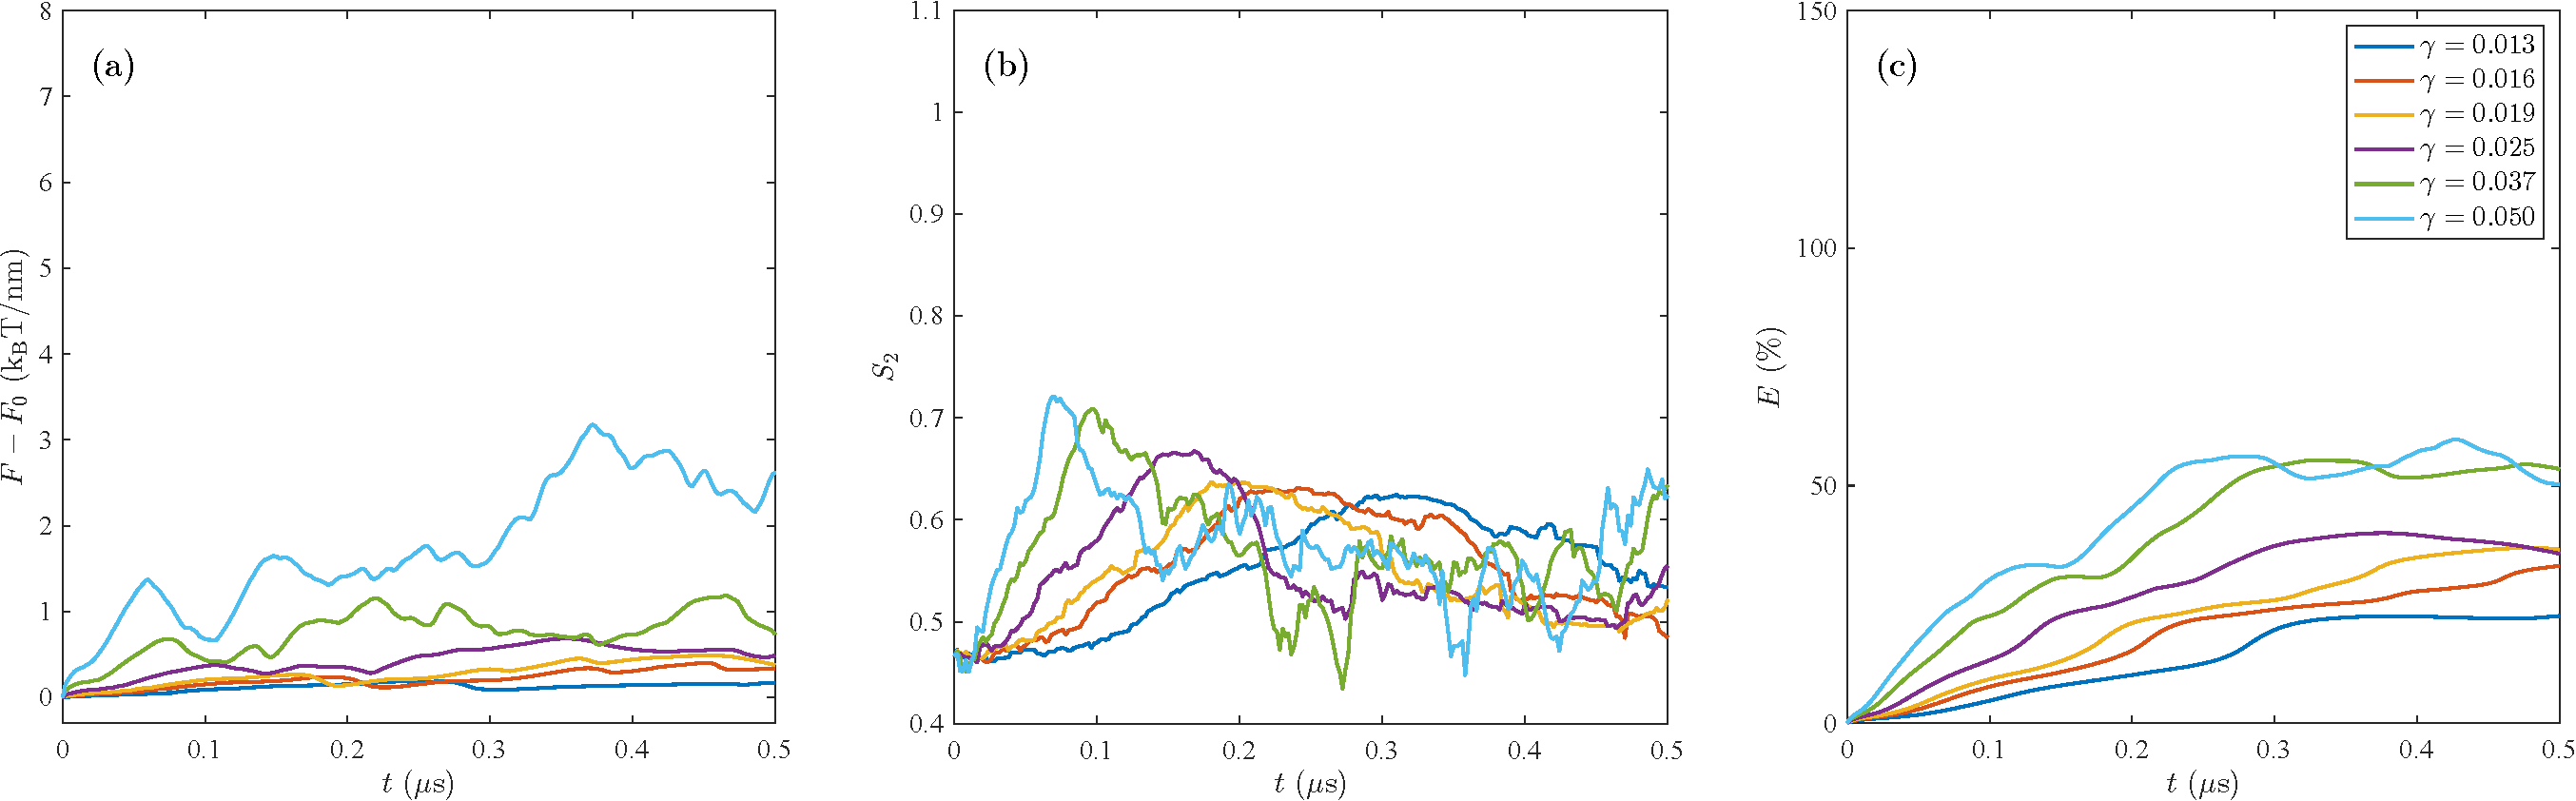
\includegraphics[width=\textwidth]{SMFigures/ULTGRaw.pdf}
\end{center}
\caption{
Relative free energy $F - F_0$,
alignment $S_2$, and strain $E$ for
Type I, bilayer phase under TG flow with choices of shear rates $\dot\gamma=0.013$ -- $0.05$ ns$^{-1}$.
%A unilamellar JP structure under a TG flow with choices of shear rates $\dot\gamma=0.013\sim0.05$. The change in free energy $F$ is plotted in panel (a). Panel (b) shows the scalar order parameter $S_2$ over time $t$. Panel (c) plots the change of strain parameter $E$ in percentage over time $t$.
}
\label{fig:ultgraw}
\end{figure}


\begin{figure}[h!]
\begin{center}
\textbf{Type I, vesicle BL phase under TG flow}\par\medskip
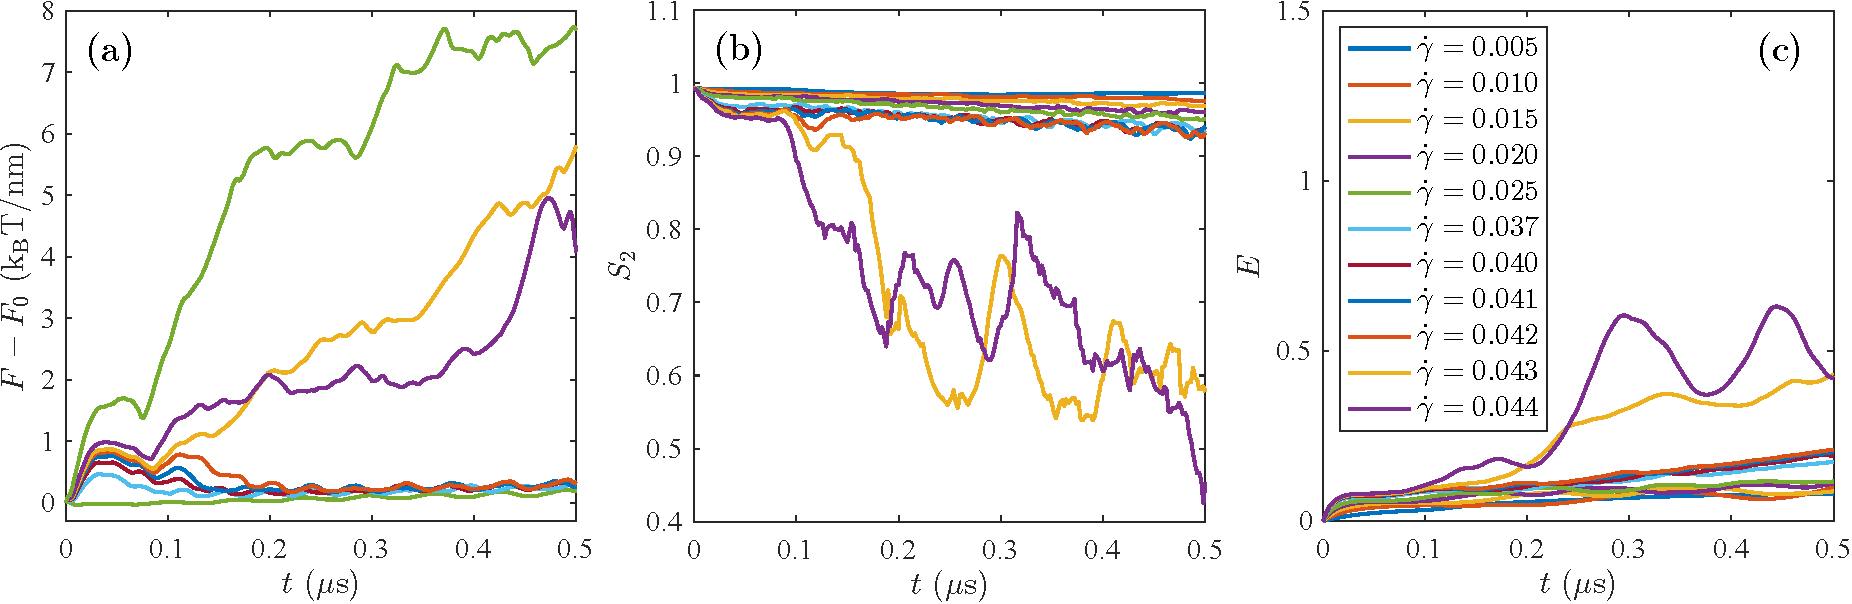
\includegraphics[width=\textwidth]{SMFigures/VeTGRaw.pdf}
\end{center}
\caption{
Relative free energy $F - F_0$,
alignment $S_2$, and strain $E$ for
Type I, vesicle bilayer phase under TG flow with choices of shear rates $\dot\gamma=0.005$ -- $0.044$ ns$^{-1}$.
The JP type is the same as for Supplementary Figure \ref{fig:ultgraw} but with a
ring-shaped, rather than disordered, bilayer for initial configuration.  
%A vesicle JP structure under a TG flow with choices of shear rates $\dot\gamma=0.005\sim0.044$. The change in free energy $F$ is plotted in panel (a). Panel (b) shows the scalar order parameter $S_2$ over time $t$. Panel (c) plots the change of strain parameter $E$ in percentage over time $t$.
}
\label{fig:vetgraw}
\end{figure}




\begin{figure}[h!]
\begin{center}
\textbf{Type II, multilamellar phase under TG flow}\par\medskip
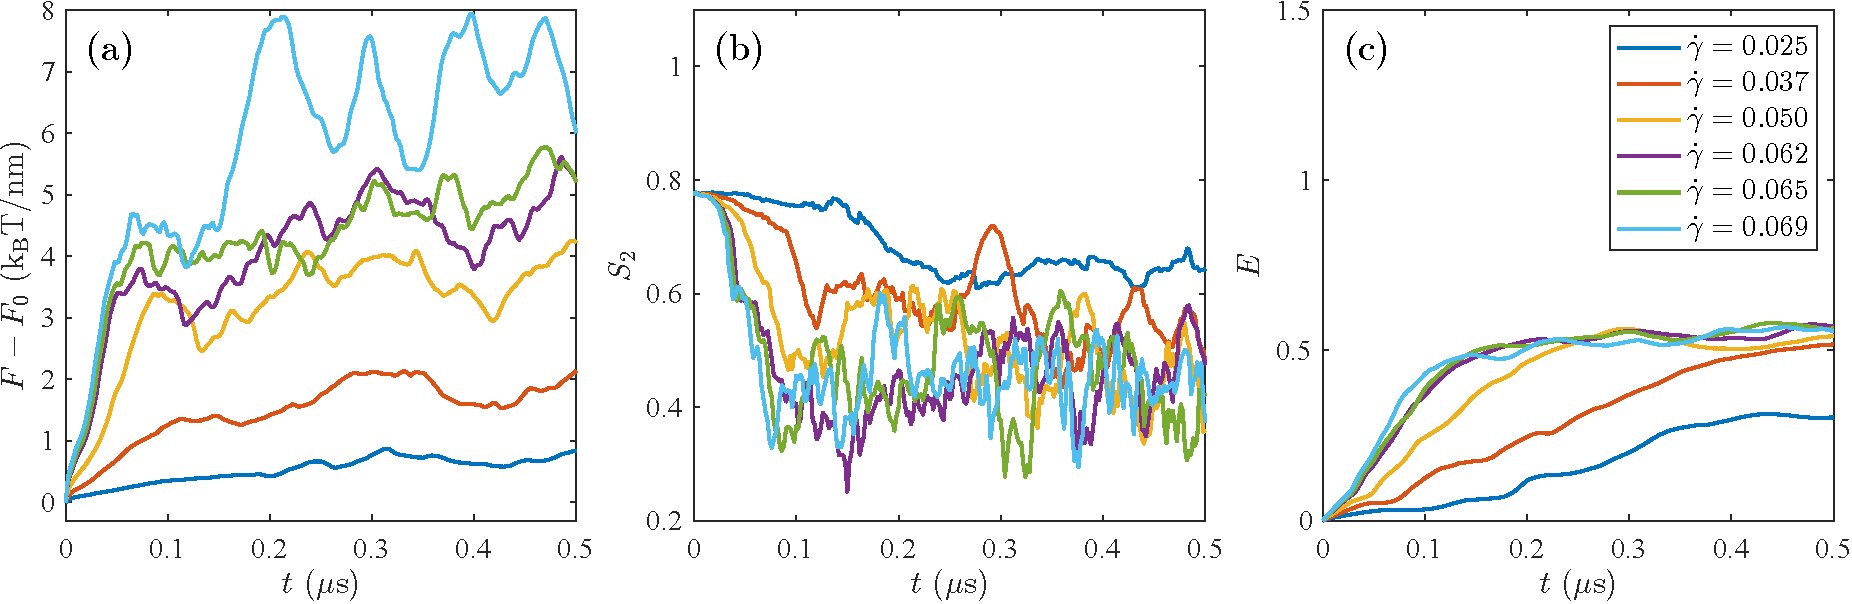
\includegraphics[width=\textwidth]{SMFigures/MLTGRaw.pdf}
\end{center}
\caption{
Relative free energy $F - F_0$,
alignment $S_2$, and strain $E$ for
Type II, multilamellar phase under TG flow with choices of shear rates $\dot\gamma=0.025$ -- $0.069$ ns$^{-1}$.
%A multilamellar JP structure under a TG flow with choices of shear rates $\dot\gamma=0.025\sim0.069$. The change in free energy $F$ is plotted in panel (a). Panel (b) shows the scalar order parameter $S_2$ over time $t$. Panel (c) plots the change of strain parameter $E$ in percentage over time $t$.
}
\label{fig:mltgraw}
\end{figure}


\begin{figure}[h!]
\begin{center}
\textbf{Type III, striated phase under TG flow}\par\medskip
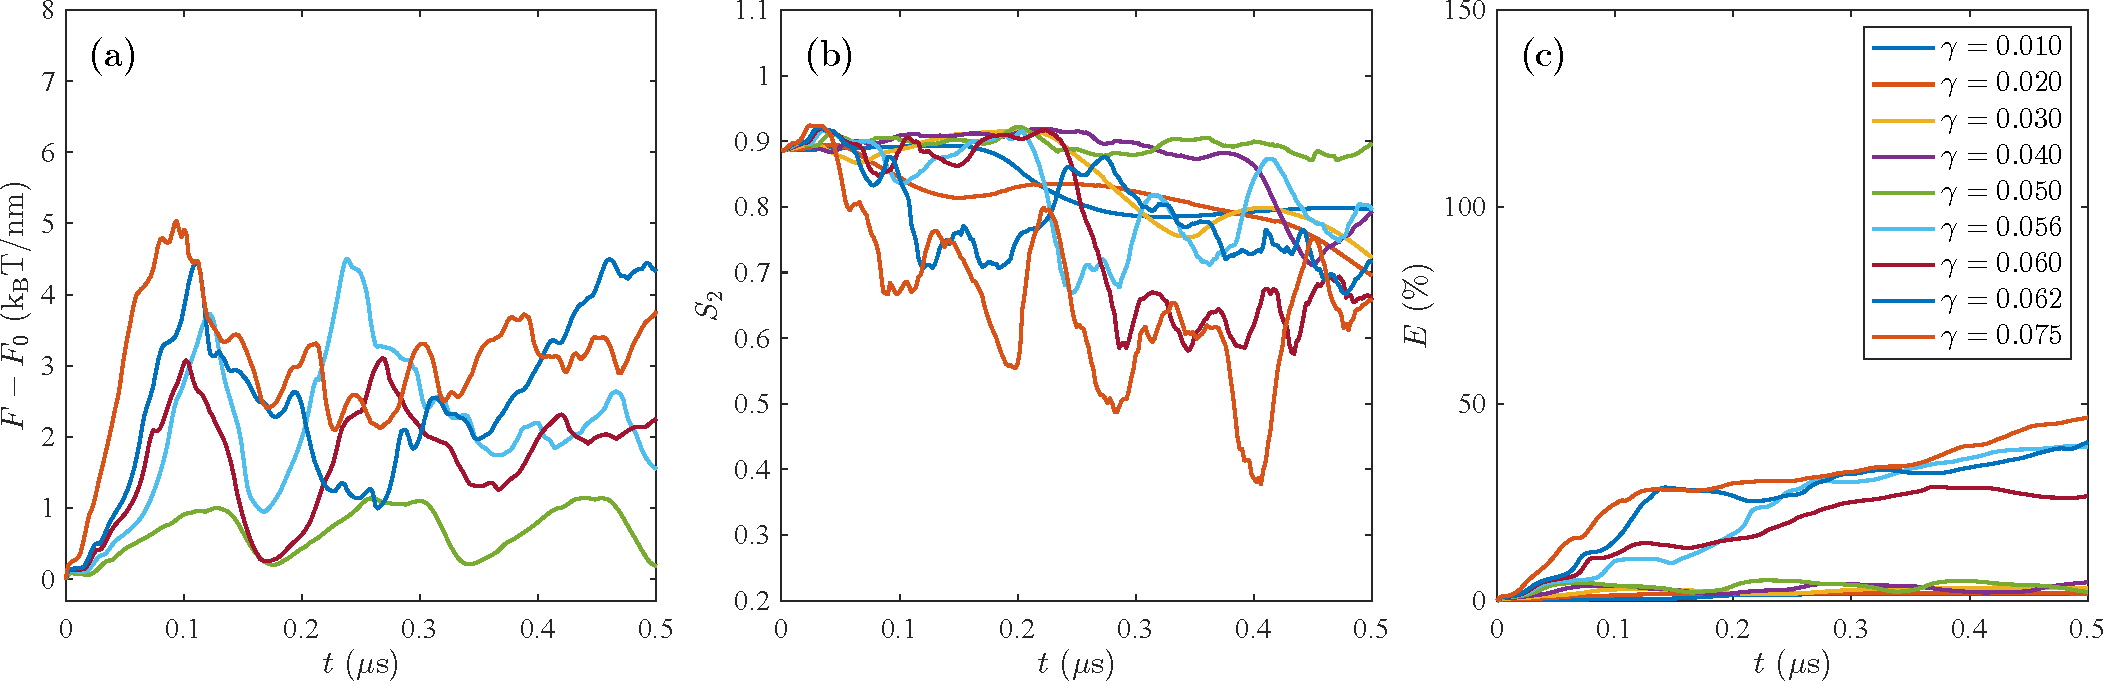
\includegraphics[width=\textwidth]{SMFigures/StTGRaw.pdf}
\end{center}
\caption{
Relative free energy $F - F_0$,
alignment $S_2$, and strain $E$ for
Type III, striated phase under TG flow with choices of shear rates $\dot\gamma=0.01$ -- $0.075$ ns$^{-1}$.
%A striated JP structure under a TG flow with choices of shear rates $\dot\gamma=0.01\sim0.069$. The change in free energy $F$ is plotted in panel (a). Panel (b) shows the scalar order parameter $S_2$ over time $t$. Panel (c) plots the change of strain parameter $E$ in percentage over time $t$.
}
\label{fig:sttgraw}
\end{figure}




